\section{Data Science - Engineering}
\todo{Demonstrate the ability for analysis.}
\todo{Link to Related works - Not repeating. Might look at the sections and link them}

\todo{Section 1 is very interesting and further supports, or cast doubts or raises question marks about what is being said in the Related works.}
The process of collecting raw data from sources, transforming it so that it matches our system's requirements and loading it into a data-set is know as \textbf{ETL.} This \textit{acronym} represents \textit{Extract - Transform - Load.}

\begin{figure}[h!]
	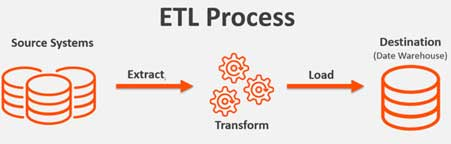
\includegraphics[width=\textwidth,height=\textheight,keepaspectratio]{fig/etl.jpg}
	\caption{Extract Transform Load.}
	\label{fig:ETL}
\end{figure}

Figure \ref{fig:ETL} shows the ETL process.


This raw data set contains lots of columns which are not necessary. The next step will be to clean the data by dropping these unnecessary columns. 


\subsection{Data Extraction.}

As mentioned in the previous chapter, the source of data for the purpose of this thesis was the Food and Agriculture Organization of the United Nations. To achieve my goals I focused on the \textbf{Value Of Agricultural Production} and in particular the \textbf{Gross Production Value.} This value was gotten by multiplying agricultural gross production by the output prices. In the data-sets used in this thesis paper, the gross production value is expressed in US dollars. 


Different data sets are available separately. For the purpose of this thesis, I narrowed down on wheat. I adopted a consistent time-frame (\textbf{1965 to 2002}). The approach to this was: \textit{Given a set of features that are consistent with a particular agricultural product, the aim is to predict the Gross Production Value.}

To make the downloaded data set globally available, I uploaded it to my GitHub repository.\cite{adeyemo_2020}

\begin{lstlisting}[language=Python]
	url_wheatArea = 'https://raw.githubusercontent.com/k-plasma/Machine-Learning-Models-for
	-Agricultural-Data-Applications/master/wheatArea.csv'	
	
	url_wheatGrossProduction = 'https://raw.githubusercontent.com/k-plasma/Machine-Learning-Models-for
	-Agricultural-Data-Applications/master/wheatGrossProductionValue.csv'	
	
	url_wheatProductionQuantity = 'https://raw.githubusercontent.com/k-plasma/Machine-Learning-Models-for
	-Agricultural-Data-Applications/master/wheatProductionQuantity.csv'	
	
	url_wheatYield = 'https://raw.githubusercontent.com/k-plasma/Machine-Learning-Models-for
	-Agricultural-Data-Applications/master/wheatYield.csv'
\end{lstlisting}

\begin{figure}[h!]
	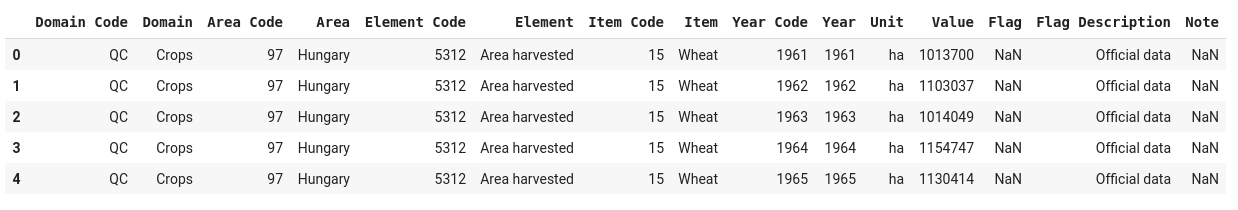
\includegraphics[width=\textwidth,height=\textheight,keepaspectratio]{fig/Area_Head.png}
	\caption{Raw Data Area.}
	\label{fig:Areaa_Head1}
\end{figure}

Figure \ref{fig:Areaa_Head1} shows the top 5 rows of the Data Set.


Each set of data set contained lots of columns which are repetitive and irrelevant to the task at hand. These columns include: \textit{"Domain Code","Domain",
	"Area Code","Area","Element Code","Element","Item Code","Item",
	"Year Code","Unit","Flag","Flag Description","Note"}

\subsection{Data Cleaning} 
The repetitive columns constitute noise which isn't required. I drop these to narrow down on the vital data necessary for my task. Two columns are left: \textit{"Year", "Value".} Since the word \textit{"Value"} appears in the different data-sets, it's renamed here as \textit{"Area(Hectares)"} to clearly indicate that this value refers to the measurement of the area.


\begin{lstlisting}[language=Python]
	df_wheatArea.drop(columns=["Domain Code","Domain",
	"Area Code","Area","Element Code","Element","Item Code","Item",
	"Year Code","Unit","Flag","Flag Description","Note"], axis=1, inplace=True)
	
	df_wheatArea.columns = ['Year', 'Area(Hectares)'] 
	
	df_wheatArea.head()
\end{lstlisting}

A similar transformation is performed on the other data-sets. The resulting individual data-sets are: 
\begin{figure}
	\centering
	\begin{subfigure}{.25\textwidth}
		\centering
		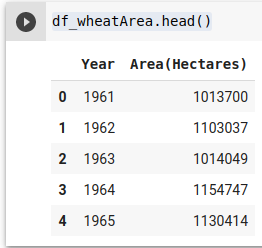
\includegraphics[width=.4\linewidth]{fig/areaHectares.png}
		\caption{Area}
		\label{fig:sub1}
	\end{subfigure}%
	\begin{subfigure}{.24\textwidth}
		\centering
		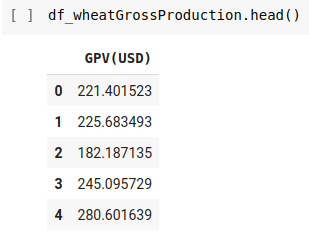
\includegraphics[width=.4\linewidth]{fig/gpv.png}
		\caption{G.P.V}
		\label{fig:sub2}
	\end{subfigure}
	\begin{subfigure}{.25\textwidth}
		\centering
		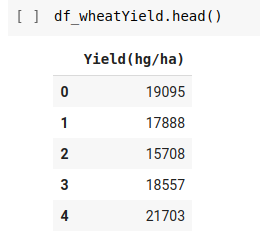
\includegraphics[width=.4\linewidth]{fig/yield.png}
		\caption{Yield}
		\label{fig:sub3}
	\end{subfigure}
	\begin{subfigure}{.24\textwidth}
		\centering
		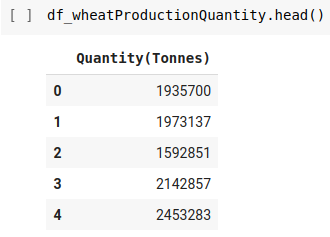
\includegraphics[width=.4\linewidth]{fig/quantityTonnes.png}
		\caption{Quantity}
		\label{fig:sub4}
	\end{subfigure}

	\caption{Individual Transformed Data-Sets}
	\label{fig:heads}
\end{figure}



\section{Implementing Machine Learning Work Flow}





\subsection{Assembling the Data Set}
\section{How I implemented the Neural Networks}
\section{Recurring Neural Network}
\section{Deep Learning}

\chapter{Results}
\section{Neural Networks}
In this section, I will describe the Progression from Normal Neural network to Recurring Neural Networks - RNN. In the end, I'll show that the GRU works well and I have solved what I set out to do. 
it should be here
\subsection{Subsection title}
Neural Networks and more advanced technologies. Right now we use Pandas for everything and it's enough, except when it's not. The more advanced we go into tech, the more basic the Machine Learning tools.

Some Machine Learning models are very dependent on used materials. SCI-KIT uses the most basic of Neural networks. What you'll notice from GPV-Take 1 is that you can't create modern systems with SCI-KIT because it is the highest level of abstraction.

Here, I'll need to show the results of the Google Colab Notebook - Gross Production Value 1 and the abysmal results I got using SCI-KIT

We use SCI-KIT for scaling. It implements it very well. Train - Test - Split
\cite{ponce1989engineering}
